%% chapter1.tex { Comments of Chapter Heads}
%
\chapter{Literature review}
This chapter contains a brief overview of conventional Image upsampling methods and Image Super Resolution approaches using Deep learning.
Image upsampling/Image Super Resolution is defined as increasing the spartial resolution while keeping the 2D representation of the image same. It is often used to enlarge a specific area of a picture and to remove the pixelation that results from displaying a low-resolution image over a big frame. Different  Deep learning based techniques that are used for image Super Resolution are mentioned in the Fig. \ref{fig:label2.1}
\begin{figure}[h]
    \centering
    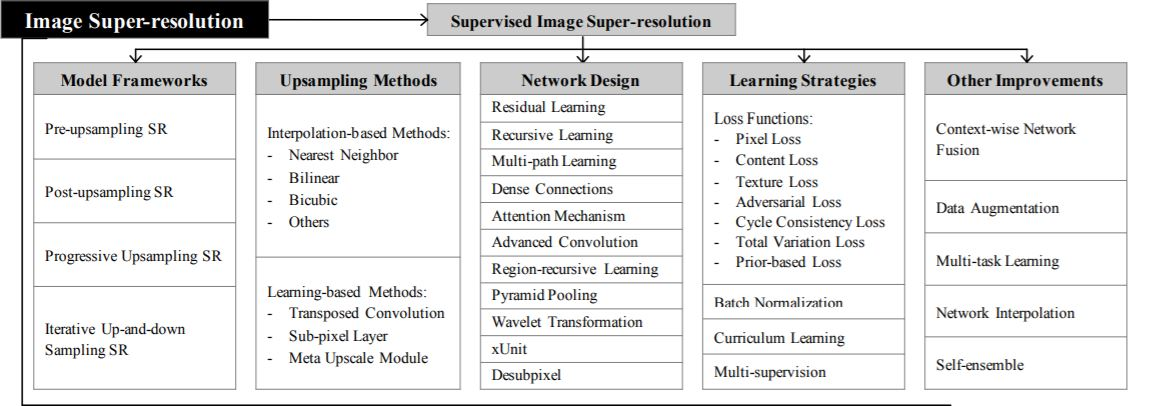
\includegraphics[totalheight=2in]{Chapter2/DLSR.jpeg}
    \caption[Techniques used for Supervised Image Super Resolution]{Techniques used for Supervised Image Super Resolution \cite{DLSR}}
    \label{fig:label2.1}
\end{figure}

\section{Image Upsampling}
Let's first comprehend upsampling (raising the spatial resolution of images or just the number of pixel rows/columns or both in the image) and its numerous techniques in order to comprehend the rest of the theory underlying super-resolution.\\
Image interpolation, also known as image scaling, is the process of resizing digital images and is frequently used in applications that deal with images. The conventional techniques include linear, bilinear, bicubic, nearest-neighbor interpolation, etc.\\
Before understanding the rest of the theory behind the super-resolution, we need to understand upsampling (Increasing the spatial resolution of images or simply increasing the number of pixel rows/columns or both in the image) and its various methods.\\

Interpolation-based methods – Image interpolation (image scaling), refers to resizing digital images and is widely used by image-related applications. The traditional methods include nearest-neighbor interpolation, linear, bilinear, bicubic interpolation.\\

Nearest-neighbor Interpolation – The nearest-neighbor interpolation is a simple and intuitive algorithm. It selects the value of the nearest pixel for each position to be interpolated regardless of any other pixels.\\

Bilinear Interpolation – The bilinear interpolation (BLI) first performs linear interpolation on one axis of the image and then performs on the other axis. Since it results in a quadratic interpolation with a receptive field-sized 2 × 2, it shows much better performance than nearest-neighbor interpolation while keeping a relatively fast speed.\\

Bicubic Interpolation – Similarly, the bicubic interpolation (BCI) performs cubic interpolation on each of the two axes Compared to BLI, the BCI takes 4 × 4 pixels into account, and results in smoother results with fewer artifacts but much lower speed. Refer to this for a detailed discussion.\\

\subsection{Learning-based upsampling}
To overcome the shortcomings of interpolation-based methods and learn upsampling in an end-to-end manner, transposed convolution layer and sub-pixel layer are introduced into the SR field.The blue boxes denote the input, and the green boxes indicate the kernel and the convolution output.

\begin{figure}[h]
    \centering
    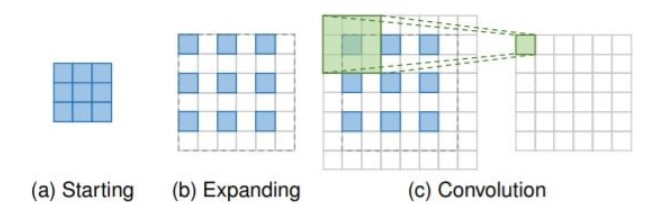
\includegraphics[totalheight=1.5in]{Chapter2/up.jpg}
    \caption[Transpose Convolution]{Transpose Convolution  \cite{DLSR}}
    \label{fig:label2.2}
\end{figure}
Transposed convolution layer, i.e. deconvolution layer, tries to perform transformation opposite a normal convolution, i.e., predicting the possible input based on feature maps sized like convolution output. Specifically, it increases the image resolution by expanding the image by inserting zeros and performing convolution.
\begin{figure}[h]
    \centering
    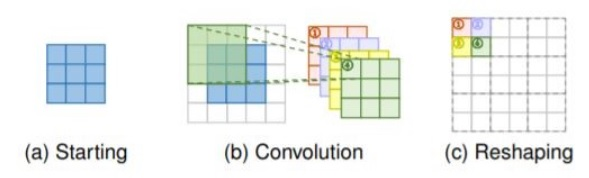
\includegraphics[totalheight=1.5in]{Chapter2/Transposed.jpg}
    \caption[Sub-pixel Layer]{Sub-pixel Layer \cite{DLSR}}
    \label{fig:label2.3}
\end{figure}
The blue boxes denote the input and the boxes with other colors indicate different convolution operations and different output feature maps.\\
Sub-pixel Layer: The sub-pixel layer, another end-to-end learnable upsampling layer, performs upsampling by generating a plurality of channels by convolution and then reshaping them shows. Within this layer, a convolution is firstly applied for producing outputs with
s2 times channels, where s is the scaling factor. Assuming the input size is h × w × c, the output size will be h×w×s2c. After that, the reshaping operation is performed to produce outputs with size sh × sw × c.\\

\section{Super-Resolution Frameworks}
Since image super-resolution is an ill-posed problem, how to perform upsampling (i.e., generating HR output from LR input) is the key problem. There are mainly four model frameworks based on the employed upsampling operations and their locations in the model (refer to the table above).\\

1. Pre-upsampling Super-resolution – It does’t make a direct mapping of LR images to HR images since it is considered to be a difficult task. It utilizes traditional upsampling algorithms to obtain higher resolution images and then refining them using deep neural networks is a straightforward solution. For example – LR images are upsampled to coarse HR images with the desired size using bicubic interpolation. Then deep CNNs are applied to these images for reconstructing high-quality images.
\begin{figure}[h]
    \centering
    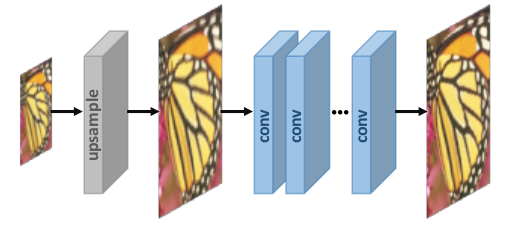
\includegraphics[totalheight=1.4in]{Chapter2/image15.png}
    \caption{Pre-upsampling architecture \cite{DLSR}}
    \label{fig:test6}
\end{figure}

2. Post-upsampling Super-resolution – To improve the computational efficiency and make full use of deep learning technology to increase resolution automatically, researchers propose to perform most computation in low-dimensional space by replacing the predefined upsampling with end-to-end learnable layers integrated at the end of the models. In the pioneer works of this framework, namely post-upsampling SR, the LR input images are fed into deep CNNs without increasing resolution, and end-to-end learnable upsampling layers are applied at the end of the network.
\begin{figure}[h]
    \centering
    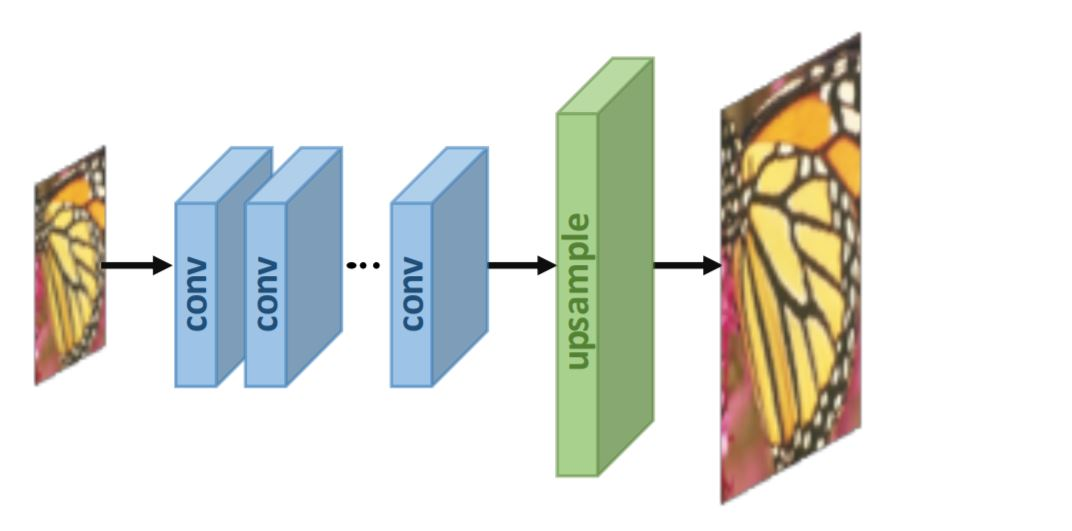
\includegraphics[totalheight=1.4in]{Chapter2/image16.jpeg}
    \caption{Post-upsampling architecture \cite{DLSR}}
    \label{fig:test7}
\end{figure}

Learning Strategies
In the super-resolution field, loss functions are used to
measure reconstruction error and guide the model optimization. In early times, researchers usually employ the pixelwise L2 loss (mean squared error), but later discover that it cannot measure the reconstruction quality very accurately. Therefore, a variety
of loss functions (e.g., content loss, adversarial loss) are adopted for better measuring the reconstruction error and producing more realistic and higher-quality results.\\
\begin{itemize}
    \item Pixelwise L1 loss – Absolute difference between pixels of ground truth HR image and the generated one.
    \item Pixelwise L2 loss – Mean squared difference between pixels of ground truth HR image and the generated one.
    \item Content loss – the content loss is indicated as the Euclidean distance between high-level representations of the output image and the target image. High-level features are obtained by passing through pre-trained CNNs like VGG and ResNet.
    \item Adversarial loss – Based on GAN where we treat the SR model as a generator, and define an extra discriminator to judge whether the input image is generated or not.
    \item PSNR – Peak Signal-to-Noise Ratio (PSNR) is a commonly used objective metric to measure the reconstruction quality of a lossy transformation. PSNR is inversely proportional to the logarithm of the Mean Squared Error (MSE) between the ground truth image and the generated image.
\end{itemize}



\subsection{Network Design}
\begin{figure}[H]
    \centering
    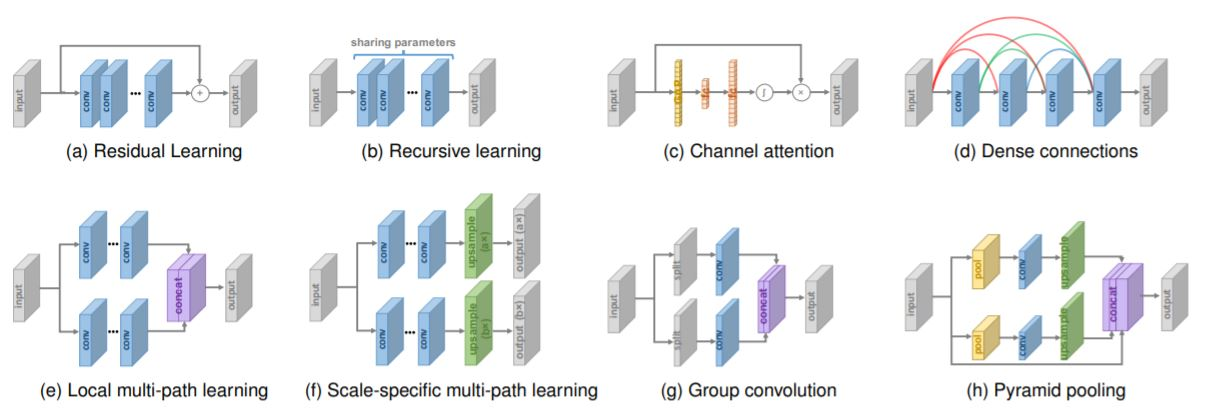
\includegraphics[totalheight=1.4in]{Chapter2/image17.jpeg}
    \caption{Various network designs in super-resolution architecture \cite{DLSR}}
    \label{fig:test8}
\end{figure}

\section{State of the Art Models}

\begin{figure}[h]
    \centering
    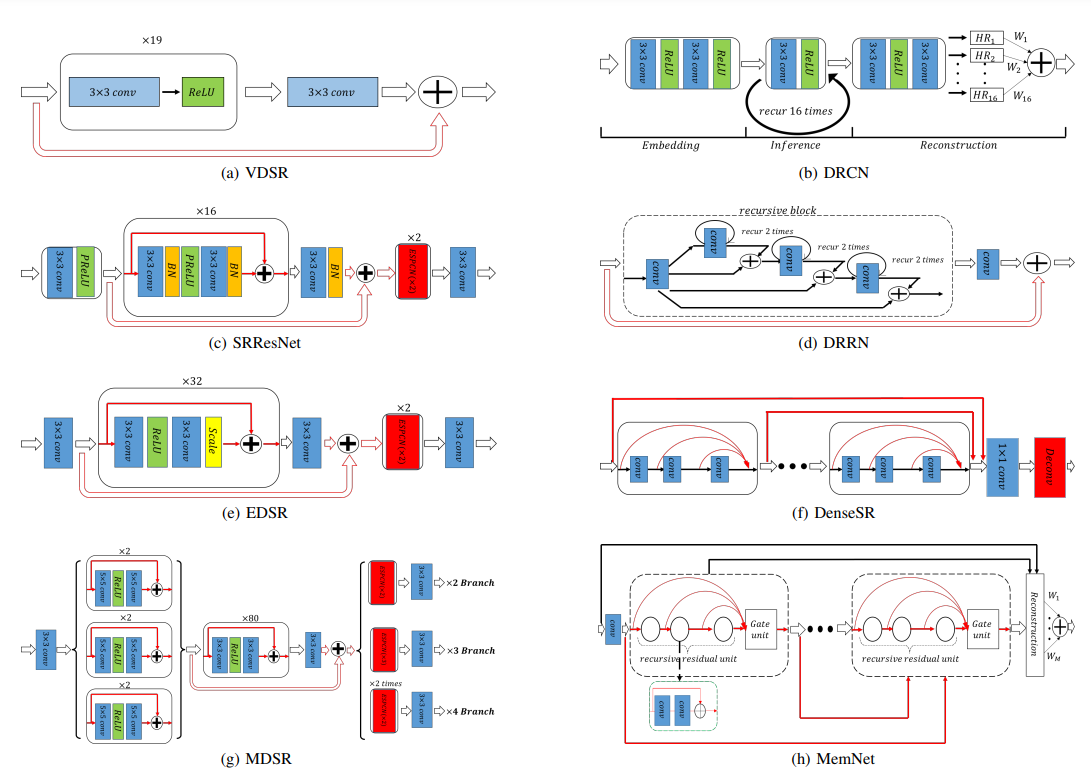
\includegraphics[totalheight=4.4in]{Chapter2/image20.png}
    \caption{Architectures of State of the Art Models \cite{DLSR}}
    \label{fig:test11}
\end{figure}
